% Copyright 2026 Sreeram Anil
% SPDX-License-Identifier: CC-BY-4.0
\chapter{Cell-level results on the equivalent-circuit plant}
\label{ch:res-cell_ecm}

\section{What is compared}

This chapter reads the cell-level benchmark across families. Every number in it comes from
the same run that produced the per-estimator tables of Parts~II--XI
(\code{results/final}, three noise seeds, eVTOL mission, equivalent-circuit plant of
\cref{ch:ecm}); the per-estimator chapters explain \emph{why} an estimator behaves as it does,
this chapter says \emph{which} of them behave alike and which do not. The metric is the
steady-state SOC RMSE of \cref{eq:me-rmsess}, in percentage points, averaged over the three
seeds; the whole-run RMSE, the peak error, the convergence time and the voltage residual of
every run are in the per-estimator tables and are quoted here where they change the reading.

\Cref{tab:overview_ecm} is the complete matrix, 70 estimators by 12 scenarios; the bold entry
marks the best of each family in each column, and \code{div} a run that met the divergence
criterion of \cref{def:me-div} in at least one seed. \Cref{fig:res-heat-ecm} is the same matrix
as a heat map on a logarithmic colour scale, which is the more useful view of it: the eye picks
out the dark cells, and the dark cells are the story. \Cref{tab:ranking} compresses each row
into a single figure of merit, the geometric mean of the twelve scenario RMSEs, which is the
ranking metric of this report because it rewards an estimator for being good everywhere and
punishes a single catastrophic column without letting it dominate.

The seed-to-seed spread matters for how finely the table can be read. Over the three seeds the
median standard deviation of $\text{RMSE}_{\text{ss}}$ is \num{0.006} percentage points in
\code{nominal}, \num{0.01}--\num{0.05} in the sensor-fault scenarios and \num{0.1}--\num{0.23}
in \code{aged\_cell}, \code{param\_mismatch} and \code{combined}. Differences of a few
hundredths of a percent between two estimators in the same column are therefore not
significant; differences of a factor of two are.

% Copyright 2026 Sreeram Anil
% SPDX-License-Identifier: CC-BY-4.0
\begingroup\scriptsize\setlength{\tabcolsep}{2.6pt}
\begin{longtable}{lrrrrrrrrrrrr}
\caption{Steady-state SOC RMSE [\%] for every estimator and scenario, ECM plant, eVTOL mission (mean over seeds). Bold: best of the family in the column; `div' marks divergence in at least one seed.}\label{tab:overview_ecm}\\
\toprule estimator & \rotatebox{60}{nominal} & \rotatebox{60}{init\_error} & \rotatebox{60}{current\_bias} & \rotatebox{60}{noise\_step} & \rotatebox{60}{outliers} & \rotatebox{60}{cold} & \rotatebox{60}{hot} & \rotatebox{60}{aged\_cell} & \rotatebox{60}{param\_mismatch} & \rotatebox{60}{sensor\_dropout} & \rotatebox{60}{preisach} & \rotatebox{60}{combined} \\ \midrule\endfirsthead
\toprule estimator & \rotatebox{60}{nominal} & \rotatebox{60}{init\_error} & \rotatebox{60}{current\_bias} & \rotatebox{60}{noise\_step} & \rotatebox{60}{outliers} & \rotatebox{60}{cold} & \rotatebox{60}{hot} & \rotatebox{60}{aged\_cell} & \rotatebox{60}{param\_mismatch} & \rotatebox{60}{sensor\_dropout} & \rotatebox{60}{preisach} & \rotatebox{60}{combined} \\ \midrule\endhead
\multicolumn{13}{l}{\textit{Baselines}} \\
\quad CoulombCounting & 0.36 & 35.35$^{\mathrm{div}}$ & 3.20 & 0.36 & 0.35 & 0.44 & 0.24 & 10.05 & 0.36 & 0.36 & \textbf{0.36} & 20.94 \\
\quad CoulombOCVHybrid & \textbf{0.17} & 4.42 & \textbf{1.94} & \textbf{0.17} & \textbf{0.05} & \textbf{0.21} & \textbf{0.24} & 9.41 & \textbf{0.16} & \textbf{0.17} & 2.28 & 1.33 \\
\quad OCVLookup & 1.30 & \textbf{1.30} & 2.13 & 1.31 & 1.31 & 1.56 & 1.24 & \textbf{1.38} & 0.41 & 1.30 & 2.15 & \textbf{1.15} \\
\multicolumn{13}{l}{\textit{Classical / sigma-point Kalman}} \\
\quad CDKF & 0.05 & 0.12 & \textbf{0.55} & 0.14 & 0.08 & 0.09 & 0.04 & 1.54 & 1.79 & 1.86 & 0.24 & 11.96 \\
\quad CKF & 0.05 & 0.09 & 0.55 & 0.15 & \textbf{0.07} & 0.11 & 0.04 & 1.79 & 1.59 & 1.92 & 0.24 & 11.26 \\
\quad CKF5 & 0.05 & 0.12 & \textbf{0.55} & 0.14 & 0.08 & 0.09 & 0.04 & 1.54 & 1.79 & 1.86 & 0.24 & 11.96 \\
\quad EIF & 0.05 & \textbf{0.05} & 0.61 & 0.12 & 0.21 & 0.16 & 0.03 & 1.52 & 1.36 & 0.46 & 0.20 & 12.44 \\
\quad EKF & 0.05 & \textbf{0.05} & 0.61 & 0.12 & 0.21 & 0.16 & 0.03 & 1.52 & 1.36 & 0.46 & 0.20 & 12.44 \\
\quad GHKF & 0.05 & 0.12 & \textbf{0.55} & 0.14 & 0.08 & 0.09 & 0.04 & 1.54 & 1.79 & 1.86 & 0.24 & 11.96 \\
\quad IEKF & 0.08 & 0.06 & 0.64 & 0.27 & 0.36 & 0.15 & 0.03 & 1.69 & 1.50 & 0.19 & 0.21 & 2.13 \\
\quad IPLF & 0.08 & 0.07 & 0.57 & 0.19 & 0.26 & 0.50 & \textbf{0.02} & 2.16 & \textbf{0.53} & 0.79 & \textbf{0.20} & 1.72 \\
\quad LKF & 1.19 & 2.19 & 1.36 & 1.19 & 1.19 & 12.49 & 1.62 & \textbf{1.14} & 1.19 & 1.20 & 1.06 & 7.00 \\
\quad SCKF & 0.05 & 0.09 & 0.55 & 0.15 & \textbf{0.07} & 0.11 & 0.04 & 1.79 & 1.59 & 1.92 & 0.24 & 11.26 \\
\quad SO-EKF & \textbf{0.04} & 0.08 & 0.62 & 0.14 & 0.30 & 0.13 & 0.03 & 1.56 & 0.89 & \textbf{0.18} & 0.20 & 1.28 \\
\quad SR-EKF & 0.05 & \textbf{0.05} & 0.61 & 0.12 & 0.21 & 0.16 & 0.03 & 1.52 & 1.36 & 0.46 & 0.20 & 12.44 \\
\quad SR-UKF & 0.04 & 0.07 & 0.57 & \textbf{0.11} & 0.18 & \textbf{0.07} & 0.03 & 1.36 & 1.37 & 0.86 & 0.23 & \textbf{1.19} \\
\quad UD-EKF & 0.05 & \textbf{0.05} & 0.61 & 0.12 & 0.21 & 0.16 & 0.03 & 1.52 & 1.36 & 0.46 & 0.20 & 12.44 \\
\quad UKF & 0.04 & 0.07 & 0.57 & \textbf{0.11} & 0.18 & \textbf{0.07} & 0.03 & 1.36 & 1.37 & 0.86 & 0.23 & \textbf{1.19} \\
\multicolumn{13}{l}{\textit{Adaptive Kalman}} \\
\quad Fading-EKF & 0.05 & 0.05 & 0.66 & 0.16 & 0.09 & 0.25 & \textbf{0.02} & 1.78 & 1.31 & 0.05 & 0.86 & 1.18 \\
\quad Fuzzy-AKF & 0.05 & 0.08 & 0.64 & 0.05 & 0.05 & 0.20 & 0.03 & 1.25 & 0.96 & 0.06 & 0.20 & 2.56 \\
\quad IAE-AKF & \textbf{0.04} & 0.07 & 0.62 & 0.04 & 0.11 & \textbf{0.16} & 0.03 & 1.21 & 1.01 & 0.05 & \textbf{0.20} & 2.01 \\
\quad IMM & 0.04 & \textbf{0.04} & 0.62 & 0.05 & 0.08 & 0.18 & 0.03 & \textbf{0.83} & 0.96 & \textbf{0.05} & 0.20 & \textbf{1.02} \\
\quad MMAE & 0.33 & 0.36 & 0.71 & 0.38 & 0.20 & 1.23 & 0.13 & 2.12 & 1.66 & 0.58 & 0.27 & 12.56 \\
\quad STF & 0.10 & 0.10 & 0.84 & 2.34 & 1.38 & 0.36 & 0.08 & 2.68 & 1.84 & 0.10 & 0.98 & 2.71 \\
\quad SageHusa-AKF & 0.04 & 0.07 & 0.62 & \textbf{0.04} & 0.06 & 0.22 & 0.04 & 1.30 & \textbf{0.76} & 0.08 & 0.20 & 1.98 \\
\quad VB-AKF & 0.05 & 0.06 & \textbf{0.61} & 0.05 & \textbf{0.05} & 0.18 & 0.03 & 1.27 & 0.79 & 0.10 & 0.20 & 1.87 \\
\multicolumn{13}{l}{\textit{Robust / embedded Kalman}} \\
\quad Constrained-EKF & 0.05 & 0.05 & 0.61 & 0.10 & 0.21 & 0.16 & 0.03 & 1.52 & 1.36 & 0.47 & 0.20 & 11.84 \\
\quad Hinf-EKF & \textbf{0.04} & \textbf{0.03} & 0.39 & 0.20 & 0.10 & 1.45 & 0.03 & 1.06 & 1.69 & 0.93 & 0.33 & 4.88 \\
\quad Huber-EKF & 0.05 & 0.05 & 0.63 & 0.06 & 0.06 & 0.13 & 0.03 & 1.73 & 0.80 & 0.12 & 0.20 & 3.77 \\
\quad MC-EKF & 0.05 & 0.05 & 0.62 & 0.07 & 0.07 & 0.16 & 0.03 & 1.41 & 1.16 & 0.14 & 0.20 & 3.23 \\
\quad ReducedOrder-EKF & 0.07 & 0.07 & 0.85 & 0.10 & 0.08 & 0.33 & \textbf{0.02} & 2.12 & 1.53 & \textbf{0.07} & 0.99 & 1.69 \\
\quad SVSF & 0.04 & 0.04 & 0.55 & 1.71 & 1.80 & \textbf{0.11} & 0.03 & 1.02 & 1.75 & 0.58 & 0.22 & 1.91 \\
\quad Schmidt-KF & 0.46 & 0.46 & \textbf{0.33} & 1.14 & 0.83 & 1.54 & 0.21 & \textbf{0.59} & \textbf{0.45} & 0.46 & 0.55 & \textbf{1.09} \\
\quad StudentT-KF & 0.04 & 0.04 & 0.62 & \textbf{0.06} & \textbf{0.05} & 0.18 & 0.03 & 1.69 & 0.77 & 0.12 & \textbf{0.20} & 4.46 \\
\multicolumn{13}{l}{\textit{Deterministic observers}} \\
\quad AdaptiveObserver & 0.05 & \textbf{0.06} & 0.74 & 0.32 & 0.17 & 0.25 & 0.04 & \textbf{1.13} & \textbf{0.83} & 0.07 & 0.97 & \textbf{0.80} \\
\quad DOB & \textbf{0.02} & 0.24 & \textbf{0.18} & 0.22 & 0.12 & \textbf{0.02} & 0.04 & 1.98 & 1.60 & 0.14 & \textbf{0.54} & 2.35 \\
\quad ESO & 0.10 & 0.10 & 0.99 & 0.42 & 0.25 & 0.75 & 0.05 & 2.64 & 1.69 & 0.10 & 1.10 & 2.54 \\
\quad HGO & 0.08 & 0.07 & 0.85 & 0.33 & 0.17 & 0.40 & \textbf{0.04} & 2.18 & 1.49 & 0.08 & 1.00 & 2.11 \\
\quad IntervalObserver & 0.08 & 0.07 & 0.85 & 0.33 & 0.17 & 0.31 & \textbf{0.04} & 2.18 & 1.49 & 0.08 & 1.00 & 2.03 \\
\quad Luenberger & 0.08 & 0.07 & 0.85 & 0.33 & 0.17 & 0.40 & \textbf{0.04} & 2.18 & 1.49 & 0.08 & 1.00 & 2.13 \\
\quad PI-Observer & 0.11 & 0.11 & 0.99 & 0.51 & 0.37 & 0.77 & 0.05 & 2.63 & 1.59 & 0.11 & 1.08 & 1.98 \\
\quad SMO & 0.08 & 0.08 & 0.86 & 0.33 & 0.17 & 0.46 & 0.04 & 2.21 & 1.49 & 0.08 & 1.01 & 2.11 \\
\quad SMO-Adaptive & 0.08 & 0.08 & 0.86 & 0.40 & 0.17 & 0.44 & 0.04 & 2.20 & 1.49 & 0.08 & 1.01 & 2.08 \\
\quad SSKF & 0.08 & 0.07 & 0.85 & 0.33 & 0.17 & 0.31 & \textbf{0.04} & 2.18 & 1.49 & 0.08 & 1.00 & 2.03 \\
\quad SuperTwisting-SMO & 0.09 & 0.09 & 0.99 & \textbf{0.16} & \textbf{0.09} & 0.37 & 0.04 & 2.49 & 1.73 & 0.09 & 1.10 & 2.46 \\
\quad UIO & 0.07 & 0.06 & 0.71 & 0.29 & 0.13 & 0.18 & 0.05 & 1.90 & 1.37 & \textbf{0.06} & 0.88 & 1.80 \\
\multicolumn{13}{l}{\textit{Joint / dual state-parameter (SOH)}} \\
\quad AWTLS & \textbf{0.02} & \textbf{0.03} & \textbf{0.22} & \textbf{0.14} & \textbf{0.19} & \textbf{0.10} & 0.10 & 0.54 & 0.83 & 0.53 & \textbf{0.64} & 9.80 \\
\quad DualEKF & 0.08 & 0.08 & 0.79 & 0.31 & 0.34 & 0.41 & 0.07 & 0.66 & 1.94 & 0.28 & 0.94 & 2.01 \\
\quad DualUKF & 0.09 & 0.12 & 0.71 & 0.27 & 0.77 & 1.61 & \textbf{0.04} & 0.11 & 2.70 & 4.12 & 1.28 & 2.10 \\
\quad JointEKF & 0.05 & 0.07 & 0.63 & 0.43 & 0.24 & 0.12 & 0.09 & \textbf{0.05} & 1.20 & 1.42 & 0.95 & 2.58 \\
\quad JointUKF & 0.11 & 0.05 & 0.58 & 0.55 & 0.37 & 0.16 & 0.08 & 0.06 & \textbf{0.49} & 1.86 & 0.94 & \textbf{1.51} \\
\quad RLS-EKF & 0.50 & 0.49 & 0.30 & 0.48 & 0.60 & 1.03 & 0.37 & 4.23 & 0.62 & \textbf{0.16} & 0.66 & 2.00 \\
\multicolumn{13}{l}{\textit{Particle / ensemble / Gaussian-sum}} \\
\quad ETKF & 0.43 & 0.86 & 2.08 & 1.72 & 1.12 & 0.71 & 0.26 & 4.61 & \textbf{0.78} & 1.08 & 0.78 & 4.81 \\
\quad EnKF & 0.27 & 0.27 & 0.84 & 1.99 & 0.96 & 1.07 & 0.14 & \textbf{2.11} & 3.58 & 0.33 & 1.00 & 3.75 \\
\quad GSF & \textbf{0.05} & \textbf{0.10} & 0.55 & \textbf{0.09} & \textbf{0.12} & \textbf{0.15} & \textbf{0.03} & 3.12 & 2.20 & 0.10 & \textbf{0.20} & 3.33 \\
\quad PF-Auxiliary & 0.15 & 0.12 & 0.91 & 0.34 & 0.36 & 0.33 & 0.07 & 2.39 & 1.63 & 0.12 & 1.07 & 2.09 \\
\quad PF-Bootstrap & 0.16 & 0.13 & 0.87 & 0.51 & 0.36 & 0.33 & 0.08 & 2.54 & 1.72 & 0.13 & 1.08 & 2.76 \\
\quad PF-Fast & 0.18 & 0.18 & 0.91 & 0.68 & 0.39 & 0.57 & 0.14 & 2.62 & 1.75 & 0.20 & 1.00 & 2.52 \\
\quad PF-Regularized & 0.12 & 0.11 & 0.90 & 0.50 & 0.34 & 0.24 & 0.06 & 2.51 & 1.88 & 0.12 & 1.00 & 2.51 \\
\quad RBPF & 0.06 & 0.35 & \textbf{0.12} & 1.12 & 0.68 & 0.18 & 0.07 & 2.25 & 1.53 & \textbf{0.07} & 0.40 & \textbf{2.05} \\
\quad UPF & 0.38 & 0.41 & 0.99 & 0.86 & 0.61 & 0.74 & 0.29 & 2.74 & 1.81 & 0.49 & 1.16 & 2.64 \\
\multicolumn{13}{l}{\textit{Data-driven}} \\
\quad ELM-RLS-EKF & \textbf{0.03} & \textbf{0.06} & \textbf{0.64} & \textbf{0.10} & \textbf{0.24} & \textbf{0.06} & \textbf{0.02} & 1.49 & 1.55 & \textbf{0.37} & 0.20 & 12.43 \\
\quad NN-Direct & 1.17 & 1.17 & 1.27 & 1.31 & 1.21 & 0.69 & 0.30 & 1.76 & 1.17 & 1.17 & 0.82 & \textbf{4.09} \\
\quad NN-EKF & 0.28 & 0.28 & 0.82 & 0.29 & 0.30 & 0.19 & 0.43 & \textbf{1.44} & \textbf{0.78} & 0.45 & \textbf{0.10} & 9.58 \\
\multicolumn{13}{l}{\textit{Moving-horizon estimation}} \\
\quad MHE & 0.11 & \textbf{0.10} & \textbf{0.09} & \textbf{0.98} & \textbf{0.49} & 0.77 & 0.04 & 0.79 & \textbf{1.98} & \textbf{0.41} & \textbf{0.46} & 0.69 \\
\quad MHE-RTI & \textbf{0.08} & 0.11 & 0.10 & 1.23 & 0.70 & \textbf{0.76} & \textbf{0.04} & \textbf{0.71} & 2.19 & 0.43 & 0.46 & \textbf{0.50} \\
\multicolumn{13}{l}{\textit{Smoothers (offline)}} \\
\quad Batch-NLS & 0.04 & 0.04 & 0.41 & 0.07 & \textbf{0.07} & 0.17 & 0.02 & 1.94 & 1.35 & \textbf{0.09} & 0.48 & 4.97 \\
\quad ERTS & 0.04 & \textbf{0.04} & \textbf{0.41} & 0.07 & 0.20 & 0.12 & \textbf{0.02} & 1.59 & \textbf{1.32} & 0.30 & 0.43 & 11.00 \\
\quad FixedLag-EKF & \textbf{0.04} & 0.04 & 0.58 & 0.12 & 0.23 & 0.14 & 0.03 & \textbf{1.55} & 1.33 & 0.43 & \textbf{0.22} & 12.41 \\
\quad URTS & 0.04 & 0.04 & 0.41 & \textbf{0.06} & 0.12 & \textbf{0.10} & 0.02 & 1.68 & 1.35 & 0.59 & 0.49 & \textbf{0.67} \\
\bottomrule\end{longtable}\endgroup


\begin{figure}[H]\centering
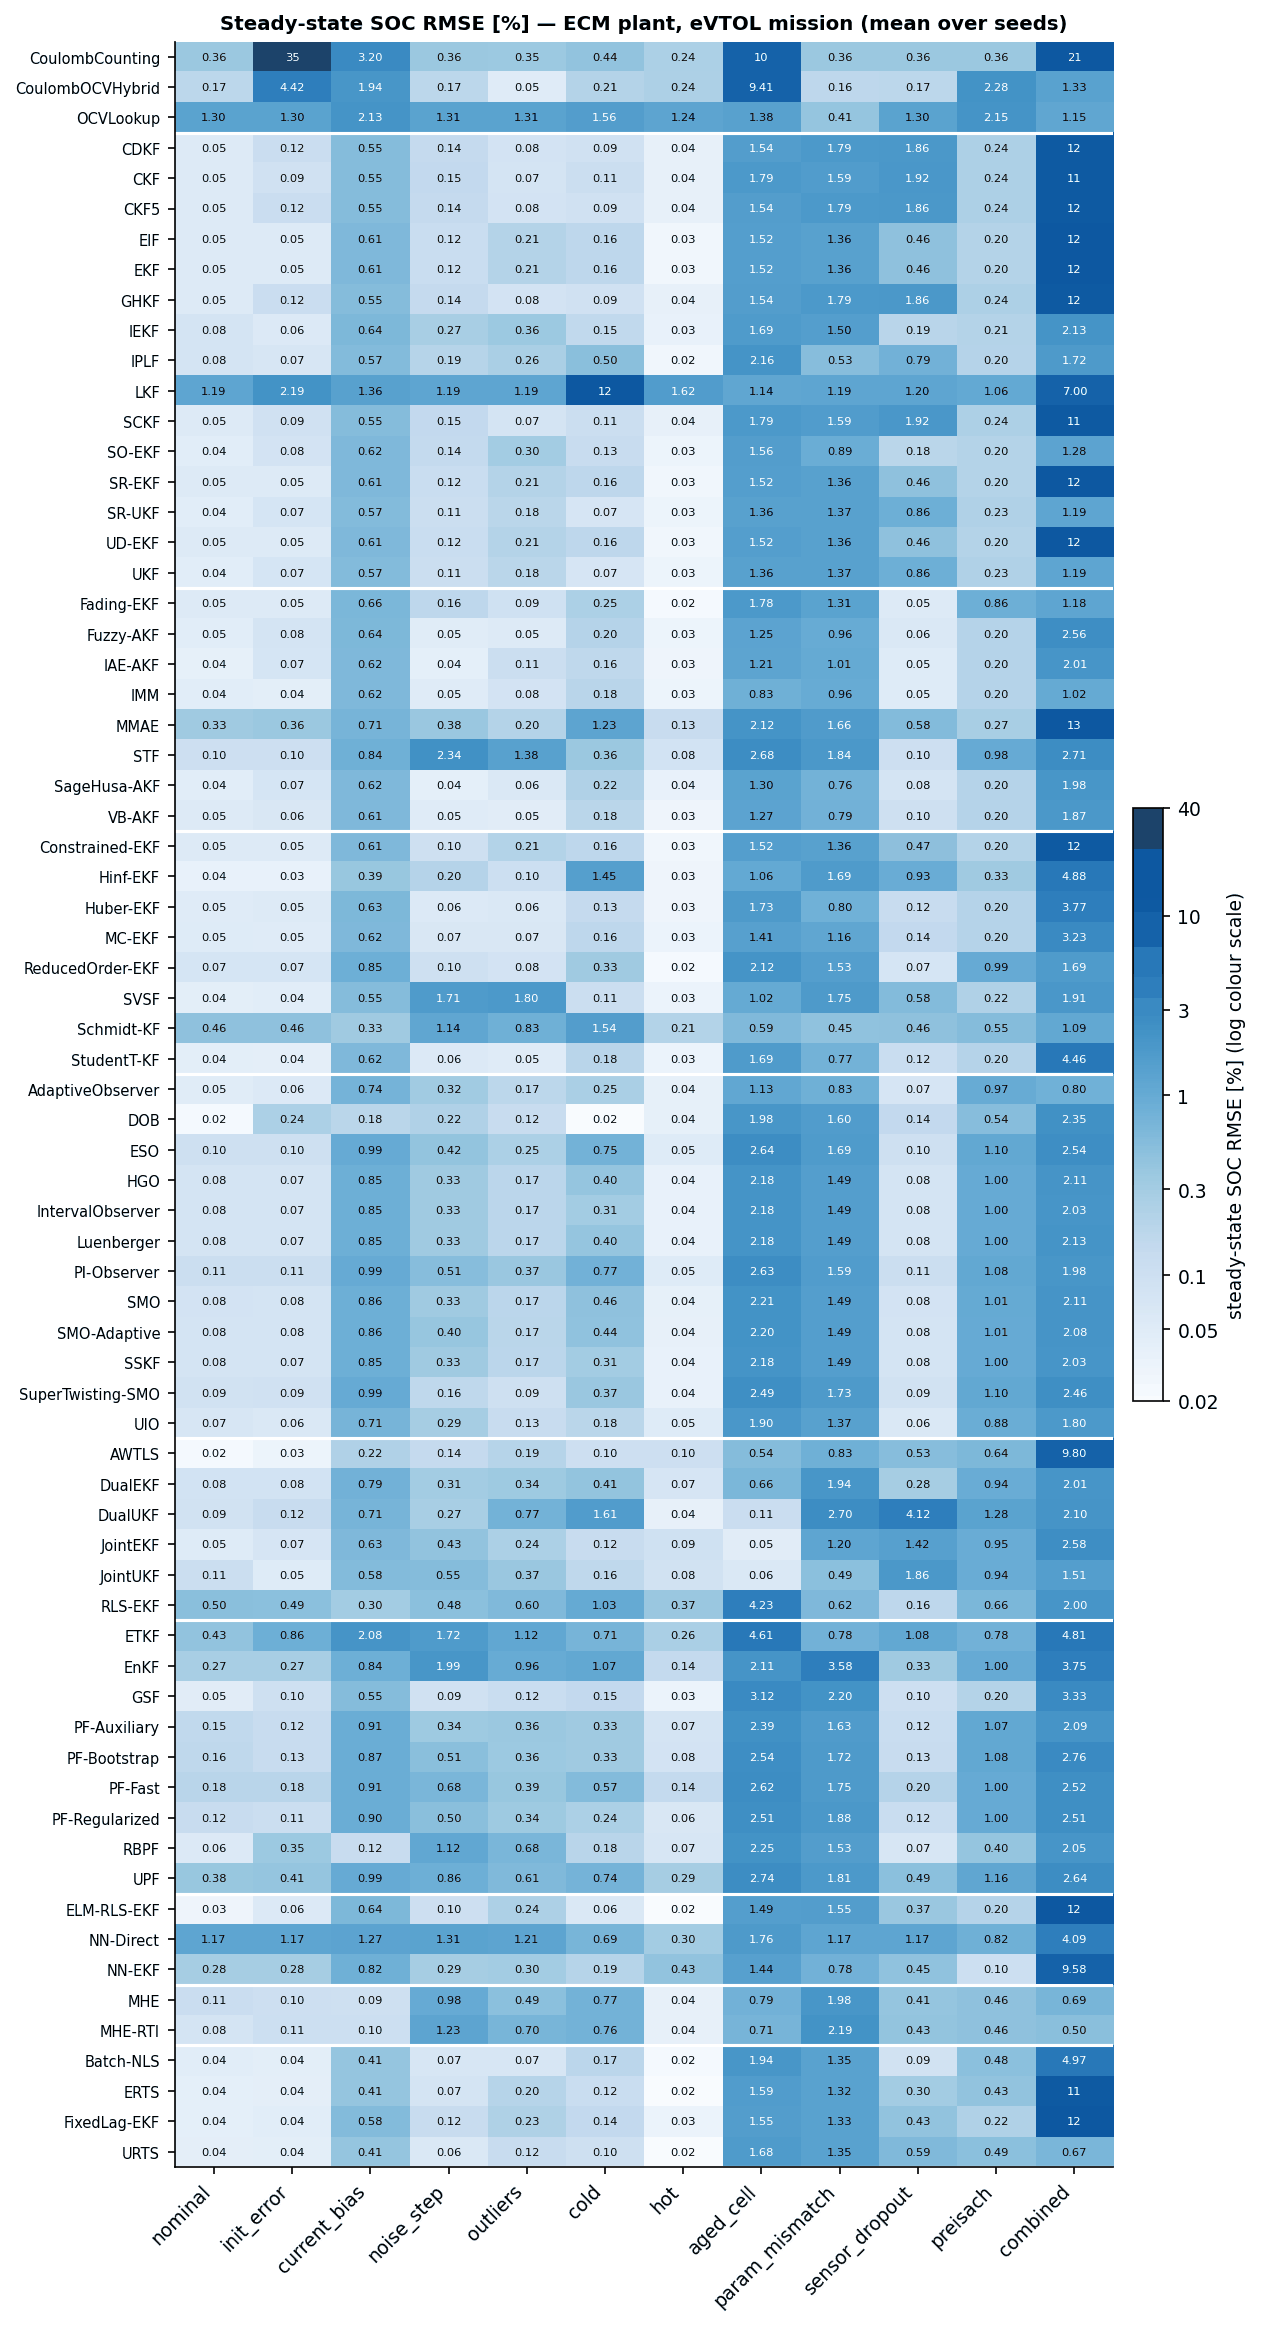
\includegraphics[width=0.98\textwidth]{figures/overview_heatmap_ecm.png}
\caption{The matrix of \cref{tab:overview_ecm} as a heat map (log colour scale). The columns
that separate the field are \code{current\_bias}, \code{aged\_cell}, \code{param\_mismatch}
and \code{combined}; the dark band in the \code{combined} column is the group of
tangent-linearised Kalman filters and their algebraic equivalents, which all fail it by the same
mechanism.}
\label{fig:res-heat-ecm}
\end{figure}

\section{The nominal floor}

On the nominal mission 51 of the 70 estimators end the flight with a steady-state RMSE below
\SI{0.1}{\percent} of capacity, i.e.\ below \SI{5}{\milli\ampere\hour}, and 66 are below
\SI{0.5}{\percent}. The floor is not the estimator's; it is the sensor's. The nominal current
sensor carries a \SI{20}{\milli\ampere} offset and a \SI{0.5}{\percent} scale-factor error
(\cref{tab:ds-sensors}), which integrate over the \SI{33.5}{\minute} mission to the
\SI{0.36}{\percent} that open-loop Coulomb counting reports, and every closed-loop estimator
removes most of that through the voltage. What remains,
\num{0.02}--\num{0.05}\,\%, is the residual of a \SI{2}{\milli\volt} voltage noise mapped
through an OCV slope of roughly \SI{0.8}{\volt} per unit SOC over the flat part of the
curve, low-pass filtered by the Kalman gain. The estimators that sit on that floor are the
EKF and everything algebraically equivalent to it (EIF, SR-EKF, UD-EKF at \num{0.05}), the
sigma-point and cubature filters (\num{0.04}--\num{0.05}), all six adaptive filters other than
MMAE and STF, the M-estimator-type robust filters (Huber, maximum-correntropy, Student's~$t$),
and the offline smoothers. The two
estimators that beat the floor, the disturbance observer and AWTLS at \SI{0.02}{\percent},
do so by estimating a bias-like quantity that absorbs the current-sensor offset; the same
property makes them the best of the field in \code{current\_bias} and, in the case of AWTLS,
the worst of the joint/dual family in \code{combined}.

The nominal column also identifies the estimators whose \emph{design} caps their accuracy.
The linear Kalman filter (\SI{1.19}{\percent}) linearises the OCV curve once, at \SI{25}{\celsius}
and mid-SOC, and pays for every departure from that point; the same frozen tangent gives it
\SI{12.49}{\percent} in \code{cold}, the worst non-divergent entry of the table. The direct
neural regressor (\SI{1.17}{\percent}) has no dynamics at all and reports the training-set
residual of its regression. The OCV inversion (\SI{1.30}{\percent}) is limited by the
first-order low-pass that makes it usable under load. The Schmidt--Kalman filter
(\SI{0.46}{\percent}) and RLS-EKF (\SI{0.50}{\percent}) deliberately \emph{under}-weight the
voltage --- the first by carrying the impedance parameters as consider states whose uncertainty
inflates the innovation covariance, the second by letting a recursive least-squares stage
absorb part of the residual --- and their nominal cost is the premium they pay for the
robustness they show in \code{param\_mismatch} and \code{aged\_cell}. MMAE
(\SI{0.33}{\percent}) reports a weighted mean over three capacity hypotheses spaced
\SI{0.5}{\ampere\hour} apart, and the weights never converge to a single hypothesis on a
nominal cell.

\section{The scenarios, column by column}

\paragraph{\code{init\_error} is an observability test, not a convergence-rate test.}
The estimator is handed an SOC \num{0.35} below the truth, with a prior standard deviation of
\num{0.1}. Every Kalman-type filter removes the error at the first measurement update, because
the prior is wide, the OCV slope at $\soc = 0.95$ is steep and the voltage noise is
\SI{2}{\milli\volt}: the first update has a gain of order \SI{1}{\per\volt} on the SOC channel
and the \SI{60}{\second}-dwell convergence time of \cref{def:me-conv} is $t_{\text{conv}} = 0$
for 35 of the 70 estimators and one sample later for the UKF, SR-UKF and second-order
EKF. The deterministic observers, whose gain is fixed by design at the
value that gives acceptable noise in steady state, take \SIrange{320}{350}{\second} to bring the
error inside \SI{2}{\percent}; the particle filters lie between (\SIrange{5}{155}{\second},
depending on how much of the prior their particle cloud covers); Coulomb counting, having no
correction, carries the error to the end and is the only divergent entry in the column. The
steady-state numbers of this column are consequently almost identical to \code{nominal} for
every estimator but the baselines, and the reader interested in transient behaviour should look
at the \code{combined} column and at the pack \code{large\_imbalance} scenario instead.

\paragraph{\code{current\_bias} separates the estimators that model a bias from those that do not.}
A \SI{0.25}{\ampere} offset and a \SI{2}{\percent} gain error on the current sensor are
unobservable from a single voltage in the ECM state space --- the model can explain the extra
charge as SOC --- so a state-only estimator converges to a biased SOC and the column reads
\num{0.55}--\num{0.99}\,\% for essentially the whole field. The exceptions all have a
mechanism that can separate an accumulating drift from a state error: moving-horizon
estimation (\num{0.09}/\num{0.10}), which re-fits a window of twenty-one samples jointly
instead of applying one gain at a time; the Rao--Blackwellised particle filter (\num{0.12}),
which treats the RC states exactly and leaves its particles free to follow the drift; the
disturbance observer (\num{0.18}), which carries an explicit lumped-disturbance state; AWTLS
(\num{0.22}), RLS-EKF (\num{0.30}) and the Schmidt filter (\num{0.33}), which identify or
consider a parameter that absorbs part of the offset; the $H_\infty$ filter (\num{0.39}),
whose worst-case gain is larger than the Kalman gain; and the three fixed-interval smoothers
(\num{0.41}), which see the whole record and can trade a constant offset against the OCV
trajectory. None of these removes the error entirely --- the gain error is not separable from a
capacity error on one mission --- and \cref{ch:res-recommendations} argues that a BMS should
solve this problem with a calibrated sensor rather than with an estimator.

\paragraph{\code{noise\_step} and \code{outliers} are where adaptive and robust filters earn their names.}
When the voltage noise steps from \SI{2}{} to \SI{20}{\milli\volt} at \SI{600}{\second} a filter
with a fixed $\mR$ is over-confident by a factor of one hundred in variance and its estimate
follows the noise; the plain EKF and the sigma-point filters read \num{0.11}--\num{0.15}\,\%, the
observers \num{0.16}--\num{0.51}\,\%. The four $\mR$-adapting filters (Sage--Husa, innovation-based,
variational Bayesian and fuzzy) recover the nominal figure to within \num{0.01}\,\%, the IMM
does the same by switching to its high-noise mode, and the M-estimator family (Huber,
maximum-correntropy, Student's~$t$) reaches \num{0.06}--\num{0.07}\,\% without adapting anything,
because a bounded influence function is a covariance adaptation in disguise. The two estimators
that are hurt most by the step are instructive: the strong-tracking filter (\SI{2.34}{\percent})
reads the larger innovations as a model change and \emph{raises} its gain, which is the wrong
response to sensor noise, and the SVSF (\SI{1.71}{\percent}) has a switching gain whose
amplitude is set by the innovation and chatters on noise. With \SI{5}{\percent} of samples
replaced by $\pm\SI{50}{\milli\volt}$ outliers the same ordering appears with larger
margins: VB-AKF, Student's~$t$, Fuzzy and the OCV-corrected Coulomb counter at
\num{0.05}\,\%, Sage--Husa \num{0.06}, Huber and MC-EKF \num{0.06}--\num{0.07}; the EKF at
\num{0.21}; STF \num{1.38} and SVSF \num{1.80}. The ensemble filters (EnKF \num{0.96}, ETKF
\num{1.12}) are poor on both because a small ensemble estimates the innovation covariance
from few samples and an outlier perturbs it.

\paragraph{\code{cold} and \code{hot} test the temperature model, and the temperature model is good.}
At \SI{-10}{\celsius} the ohmic resistance of the plant is about three times its
\SI{25}{\celsius} value, the slow-branch resistance five times, and the RC time constants
are nearly four times longer (\cref{ch:ecm}); every estimator is
told the temperature and uses the same Arrhenius law as the plant, so the scenario is a test of
whether the estimator copes with a slower, higher-impedance cell rather than of model error.
Most do: the sigma-point filters (\num{0.07}), the EKF (\num{0.16}), the adaptive filters
(\num{0.16}--\num{0.25}), the observers (\num{0.18}--\num{0.46} except the ESO and PI observer
at \num{0.75}), and the disturbance observer at \num{0.02}, which absorbs the higher IR drop
directly. The failures are the estimators whose gains were designed at \SI{25}{\celsius} and
not re-tuned: the linear Kalman filter (\num{12.49}), the $H_\infty$ filter, whose $\gamma$
bound is close to its feasibility limit at the nominal operating point and whose Riccati
recursion is pushed against it by the larger residuals (\num{1.45}), the Schmidt filter
(\num{1.54}) and the dual UKF (\num{1.61}), and the MMAE bank (\num{1.23}), whose
likelihood ratios are distorted by the larger model residual at low temperature. \code{hot}
at \SI{45}{\celsius} is benign for everybody: the impedance is lower, the model residual is
smaller, and 56 of the 70 estimators read \num{0.1}\,\% or better.

\paragraph{\code{aged\_cell}: only a capacity estimator fixes a capacity error.}
The plant has lost \SI{15}{\percent} of its capacity and gained \SI{37.5}{\percent} ohmic
resistance; the estimator is told neither. The column is the cleanest family separation in the
table. The joint and dual filters that carry capacity as a state read \num{0.05} (joint EKF),
\num{0.06} (joint UKF), \num{0.11} (dual UKF), \num{0.54} (AWTLS) and \num{0.66} (dual EKF).
Every state-only estimator is an order of magnitude worse, because a wrong capacity biases
the Coulomb-counting prediction at every step and the voltage correction can only pull the
estimate back at the rate its gain allows: the best state-only results are the Schmidt filter
(\num{0.59}, which treats capacity as a consider parameter and so keeps a gain large enough to
follow), the IMM (\num{0.83}, whose modes span two capacity hypotheses), the SVSF (\num{1.02})
and the $H_\infty$ filter (\num{1.06}); the EKF reads \num{1.52}, the observers
\num{1.9}--\num{2.6}, the particle filters \num{2.1}--\num{4.6}. RLS-EKF, which identifies
resistance but not capacity, is the worst of its family at \num{4.23} because the identified
resistance absorbs part of the error that belongs to the capacity.

\paragraph{\code{param\_mismatch}: a voltage-model error is best handled by trusting the voltage less.}
The estimator's $R_0$ is \SI{30}{\percent} low, $R_1$ \SI{30}{\percent} high and $\tau_2$
\SI{50}{\percent} long. The remarkable entries are at the top of the table: the OCV-corrected
Coulomb counter (\num{0.16}) and plain Coulomb counting (\num{0.36}) beat every model-based
filter, because the mismatch lives entirely in the voltage model and an estimator that
integrates current under load and only consults the voltage at rest, or never, is immune to
it. Among the closed-loop estimators the winners are those that discount the voltage: the
Schmidt filter (\num{0.45}), the joint UKF (\num{0.49}, which re-identifies part of the error),
the iterated posterior linearisation filter (\num{0.53}), RLS-EKF (\num{0.62}) and the
$\mR$-adapting and M-estimator filters (\num{0.76}--\num{0.80}), which read the structured residual
as noise and lower their gain. The EKF and the UKF read \num{1.36}--\num{1.37}, the cubature and
central-difference filters \num{1.6}--\num{1.8} (the wider point set turns the impedance error
into a larger effective OCV-slope error, as \cref{ch:ckf} explains), the observers
\num{1.4}--\num{1.7}, EnKF \num{3.58}.

\paragraph{\code{sensor\_dropout}: fifteen seconds of a stuck voltage channel.}
At \SI{200}{\second} the voltage measurement freezes for \SI{15}{\second} while the current
continues to change. A filter that believes the measurement drives its SOC to explain a constant
voltage under a varying load, collapses its covariance in the process, and must then recover
from a wrong, confident state; the steady-state column measures how much of the damage is
still present in the second half of the flight. The estimators that gate the innovation or
adapt the measurement noise are unaffected (Fading-EKF, IMM, IAE-AKF \num{0.05}; Fuzzy-AKF,
UIO \num{0.06}; reduced-order EKF, RBPF \num{0.07}), and so are the fixed-gain observers
(\num{0.08}--\num{0.11}), whose gain is too small to be dragged far in fifteen seconds. The
EKF is left with \num{0.46}, the UKF with \num{0.86} and the third-degree cubature and
Gauss--Hermite filters with \num{1.86}--\num{1.92}: a wide prior after the dropout makes the
statistical linearisation of the OCV curve steeper than the tangent, and the recovery is
mis-scaled. The dual UKF (\num{4.12}) attributes the stuck voltage to a capacity change.

\paragraph{\code{preisach}: the one-state hysteresis model is adequate.}
With the plant's hysteresis replaced by a 32-level Preisach operator of \SI{15}{\milli\volt}
amplitude, against the estimator's one-state model with $M = \SI{5}{\milli\volt}$, the Kalman
family reads \num{0.20}--\num{0.24}\,\%, the NN-EKF \num{0.10} (its residual network was trained on
Preisach cells, which is also why it is worse than the EKF on a cell without the loop), the fixed-gain observers, the sampling particle filters and the joint and dual filters
\num{0.9}--\num{1.3}, and the baselines \num{2.2}; the exceptions in those families are the
estimators with a free slow state or an exact RC marginal --- the disturbance observer
(\num{0.54}), the RBPF (\num{0.40}) and the Gaussian-sum filter (\num{0.20}). The Kalman
filters absorb the unmodelled part of the loop in the slow RC state, which is available for
that purpose; the observers, with a fixed gain distribution across the state, cannot. The magnitude of the effect is a \SI{10}{\milli\volt}
modelling error mapped through the OCV slope, i.e.\ about \SI{1}{\percent} SOC, which is what
the estimators without a free slow state report.

\paragraph{\code{combined}: the scenario that splits the library in two.}
A \num{0.25} initial error, a \SI{0.15}{\ampere} bias with a \SI{2}{\percent} gain error, a
\SI{10}{\percent} capacity loss with its resistance growth, and \SI{0}{\celsius}. Eighteen
estimators end with a steady-state error above \SI{5}{\percent}: the EKF and its three
algebraic equivalents, the constrained EKF, the fixed-lag and fixed-interval extended smoothers,
the ELM-RLS-EKF and NN-EKF (which are EKFs with a learned correction), the third-degree
cubature family with the Gauss--Hermite and central-difference filters, MMAE, AWTLS, the linear
KF and Coulomb counting. All of them fail by the mechanism documented in \cref{ch:ekf}: the
first update collapses the SOC covariance by a factor of fifteen on the strength of a
linearisation that is not valid over a $\sigma = 0.1$ prior, the remaining \SI{7}{\percent}
error is locked in, and the aged cell's extra ohmic drop during the landing hover is then
attributed to SOC. Every estimator that keeps its prior honest survives: the UKF and SR-UKF
(\num{1.19}), the second-order EKF (\num{1.28}), the IPLF (\num{1.72}) and the IEKF
(\num{2.13}) by accounting for the OCV curvature; the fading-memory (\num{1.18}), IMM
(\num{1.02}) and $\mR$-adapting filters (\num{1.9}--\num{2.6}) by not letting the covariance
collapse; the observers (\num{1.8}--\num{2.5}) by having no covariance to collapse; and the
four best entries of the column, MHE-RTI (\num{0.50}), MHE (\num{0.69}), the adaptive
observer (\num{0.80}) and the IMM (\num{1.02}), by re-fitting a window of the record, by
adapting the resistance explicitly, or by mixing a nominal and an aged hypothesis. The joint and dual filters, which should in principle identify the
\SI{10}{\percent} capacity loss, read \num{1.5}--\num{2.6}: on a cold, biased mission the
capacity is not separately identifiable from the bias within one flight, and the multi-flight
study of \cref{ch:res-soh} is where they show their value.

\section{Mission profiles}

\Cref{tab:profiles} repeats the nominal scenario on the four missions of \cref{ch:datasets}.
The fixed-wing profile, with its long, nearly constant cruise current, and the hover-hold
profile, with a high constant current, are easier than the eVTOL profile for every estimator
whose model is right (the EKF reads \num{0.06}/\num{0.02}), because a constant current excites
nothing that the model does not describe; the eVTOL transitions are where the RC states and
the hysteresis state matter. The ground-charge profile is the interesting column. It is a
CC--CV charge with rest periods, and it exposes every estimator that identifies a parameter
from a weakly exciting signal: the joint and dual filters read \num{3.6}--\num{6.1}\,\% (AWTLS, which
anchors on discharge swings and rejects the charge, is the exception at \num{0.02}),
RLS-EKF \num{3.14}, the Schmidt filter \num{3.35}, the unknown-input observer \num{4.73} and the
direct neural regressor, which was trained on discharge missions, \num{8.86}. The state-only
Kalman filters and observers are unaffected (\num{0.02}--\num{0.1}). The practical reading is
the one that \cref{ch:res-recommendations} makes into a rule: a parameter estimator needs an
excitation gate, and a charge at constant current is not excitation.

% Copyright 2026 Sreeram Anil
% SPDX-License-Identifier: CC-BY-4.0
\begin{longtable}{lrrrr}
\caption{Steady-state SOC RMSE [\%] on the four mission profiles (nominal scenario, ECM plant).}\label{tab:profiles}\\
\toprule estimator & evtol & fixed\_wing & hover\_hold & ground\_charge \\ \midrule\endfirsthead
\toprule estimator & evtol & fixed\_wing & hover\_hold & ground\_charge \\ \midrule\endhead
CoulombCounting & 0.36 & 0.45 & 0.28 & 0.08 \\
CoulombOCVHybrid & 0.17 & 0.09 & 0.11 & 0.05 \\
OCVLookup & 1.30 & 0.78 & 1.95 & 0.55 \\
CDKF & 0.05 & 0.06 & 0.02 & 0.02 \\
CKF & 0.05 & 0.06 & 0.02 & 0.02 \\
CKF5 & 0.05 & 0.06 & 0.02 & 0.02 \\
EIF & 0.05 & 0.06 & 0.02 & 0.02 \\
EKF & 0.05 & 0.06 & 0.02 & 0.02 \\
GHKF & 0.05 & 0.06 & 0.02 & 0.02 \\
IEKF & 0.08 & 0.06 & 0.12 & 0.02 \\
IPLF & 0.08 & 0.04 & 0.09 & 0.04 \\
LKF & 1.19 & 1.73 & 6.25 & 4.05 \\
SCKF & 0.05 & 0.06 & 0.02 & 0.02 \\
SO-EKF & 0.04 & 0.03 & 0.05 & 0.04 \\
SR-EKF & 0.05 & 0.06 & 0.02 & 0.02 \\
SR-UKF & 0.04 & 0.06 & 0.03 & 0.02 \\
UD-EKF & 0.05 & 0.06 & 0.02 & 0.02 \\
UKF & 0.04 & 0.06 & 0.03 & 0.02 \\
Fading-EKF & 0.05 & 0.05 & 0.04 & 0.05 \\
Fuzzy-AKF & 0.05 & 0.06 & 0.02 & 0.02 \\
IAE-AKF & 0.04 & 0.06 & 0.02 & 0.02 \\
IMM & 0.04 & 0.06 & 0.02 & 0.02 \\
MMAE & 0.33 & 0.23 & 0.22 & 0.21 \\
STF & 0.10 & 0.15 & 0.09 & 0.18 \\
SageHusa-AKF & 0.04 & 0.06 & 0.02 & 0.02 \\
VB-AKF & 0.05 & 0.06 & 0.02 & 0.02 \\
Constrained-EKF & 0.05 & 0.06 & 0.02 & 0.02 \\
Hinf-EKF & 0.04 & 0.04 & 0.01 & 0.03 \\
Huber-EKF & 0.05 & 0.06 & 0.02 & 0.02 \\
MC-EKF & 0.05 & 0.08 & 0.02 & 0.03 \\
ReducedOrder-EKF & 0.07 & 0.07 & 0.05 & 0.04 \\
SVSF & 0.04 & 0.06 & 0.02 & 0.02 \\
Schmidt-KF & 0.46 & 0.67 & 0.48 & 3.35 \\
StudentT-KF & 0.04 & 0.06 & 0.02 & 0.02 \\
AdaptiveObserver & 0.05 & 0.05 & 0.04 & 0.07 \\
DOB & 0.02 & 0.02 & 0.02 & 0.02 \\
ESO & 0.10 & 0.09 & 0.07 & 0.10 \\
HGO & 0.08 & 0.07 & 0.06 & 0.04 \\
IntervalObserver & 0.08 & 0.07 & 0.06 & 0.04 \\
Luenberger & 0.08 & 0.07 & 0.06 & 0.04 \\
PI-Observer & 0.11 & 0.08 & 0.07 & 0.08 \\
SMO & 0.08 & 0.07 & 0.06 & 0.05 \\
SMO-Adaptive & 0.08 & 0.07 & 0.06 & 0.04 \\
SSKF & 0.08 & 0.07 & 0.06 & 0.04 \\
SuperTwisting-SMO & 0.09 & 0.08 & 0.06 & 0.06 \\
UIO & 0.07 & 0.06 & 0.06 & 4.73 \\
AWTLS & 0.02 & 0.18 & 0.02 & 0.02 \\
DualEKF & 0.08 & 0.05 & 0.09 & 6.08 \\
DualUKF & 0.09 & 0.04 & 0.35 & 3.62 \\
JointEKF & 0.05 & 0.03 & 0.03 & 3.85 \\
JointUKF & 0.11 & 0.12 & 0.11 & 3.60 \\
RLS-EKF & 0.50 & 0.22 & 2.87 & 3.14 \\
ETKF & 0.43 & 0.48 & 0.27 & 0.05 \\
EnKF & 0.27 & 0.22 & 0.19 & 0.42 \\
GSF & 0.05 & 0.06 & 0.03 & 0.02 \\
PF-Auxiliary & 0.15 & 0.16 & 0.13 & 0.23 \\
PF-Bootstrap & 0.16 & 0.18 & 0.07 & 0.35 \\
PF-Fast & 0.18 & 0.21 & 0.14 & 0.70 \\
PF-Regularized & 0.12 & 0.13 & 0.14 & 0.14 \\
RBPF & 0.06 & 0.12 & 0.03 & 0.05 \\
UPF & 0.38 & 0.43 & 0.35 & 0.76 \\
ELM-RLS-EKF & 0.03 & 0.06 & 0.08 & 0.03 \\
NN-Direct & 1.17 & 0.49 & 0.61 & 8.86 \\
NN-EKF & 0.28 & 0.55 & 0.38 & 0.95 \\
MHE & 0.11 & 0.11 & 0.16 & 0.13 \\
MHE-RTI & 0.08 & 0.10 & 0.15 & 0.11 \\
Batch-NLS & 0.04 & 0.05 & 0.03 & 0.03 \\
ERTS & 0.04 & 0.04 & 0.05 & 0.03 \\
FixedLag-EKF & 0.04 & 0.04 & 0.08 & 0.04 \\
URTS & 0.04 & 0.04 & 0.05 & 0.03 \\
\bottomrule\end{longtable}


\section{Ranking and cost}

\Cref{tab:ranking} orders the 70 estimators by the geometric mean of their twelve scenario
RMSEs. The top of the list is occupied by the adaptive family --- IMM (\num{0.16}), IAE-AKF,
VB-AKF, Sage--Husa and Fuzzy (\num{0.18}) --- followed by the M-estimator robust filters
(Student's~$t$, Huber, MC-EKF at \num{0.19}--\num{0.20}), the unscented smoother, the
disturbance observer (\num{0.22}), the fading-memory EKF (\num{0.23}) and the UKF pair
(\num{0.24}). The EKF is 27th at \num{0.30}; its rank is set entirely by the \code{combined}
column, without which it would be in the top ten. The bottom of the list holds the estimators
with a structural accuracy cap (LKF, OCV lookup, NN-Direct, Coulomb counting) and the
ensemble methods (ETKF, EnKF, UPF), whose small ensembles cannot represent a
four-dimensional posterior with a \SI{2}{\milli\volt} likelihood.

Two cautions apply to the ranking. First, the ``worst'' column is as important as the mean: the
ELM-RLS-EKF is 19th by geometric mean but has a worst case of \num{12.43}, and AWTLS is 18th
with a worst case of \num{9.80}; a certification argument is made on the worst column.
Second, the offline smoothers are listed for reference only --- they see the whole record and
are not candidates for a flight estimator.

% Copyright 2026 Sreeram Anil
% SPDX-License-Identifier: CC-BY-4.0
\begingroup\footnotesize\setlength{\tabcolsep}{4pt}
\begin{longtable}{rllrrrr}
\caption{Composite ranking of all cell-level estimators on the ECM plant: geometric-mean steady-state RMSE over the 12 scenarios (lower is better), worst-scenario RMSE, nominal RMSE and cost. Offline smoothers are listed for reference.}\label{tab:ranking}\\
\toprule rank & estimator & family & geo.-mean [\%] & worst [\%] & nominal [\%] & ns/step \\ \midrule\endfirsthead
\toprule rank & estimator & family & geo.-mean [\%] & worst [\%] & nominal [\%] & ns/step \\ \midrule\endhead
1 & IMM & adaptive\_kalman & 0.16 & 1.02 & 0.04 & 2076 \\
2 & IAE-AKF & adaptive\_kalman & 0.18 & 2.01 & 0.04 & 500 \\
3 & VB-AKF & adaptive\_kalman & 0.18 & 1.87 & 0.05 & 872 \\
4 & SageHusa-AKF & adaptive\_kalman & 0.18 & 1.98 & 0.04 & 545 \\
5 & Fuzzy-AKF & adaptive\_kalman & 0.18 & 2.56 & 0.05 & 727 \\
6 & StudentT-KF & robust\_kalman & 0.19 & 4.46 & 0.04 & 696 \\
7 & Huber-EKF & robust\_kalman & 0.19 & 3.77 & 0.05 & 642 \\
8 & URTS & smoothers & 0.20 & 1.68 & 0.04 & 2473 \\
9 & MC-EKF & robust\_kalman & 0.20 & 3.23 & 0.05 & 998 \\
10 & Batch-NLS & smoothers & 0.21 & 4.97 & 0.04 & 4662 \\
11 & DOB & observers & 0.22 & 2.35 & 0.02 & 587 \\
12 & Fading-EKF & adaptive\_kalman & 0.23 & 1.78 & 0.05 & 501 \\
13 & SO-EKF & kalman & 0.23 & 1.56 & 0.04 & 4202 \\
14 & SR-UKF & kalman & 0.24 & 1.37 & 0.04 & 1554 \\
15 & UKF & kalman & 0.24 & 1.37 & 0.04 & 1442 \\
16 & AdaptiveObserver & observers & 0.25 & 1.13 & 0.05 & 900 \\
17 & GSF & particle & 0.25 & 3.33 & 0.05 & 1749 \\
18 & AWTLS & soh & 0.25 & 9.80 & 0.02 & 483 \\
19 & ELM-RLS-EKF & learning & 0.25 & 12.43 & 0.03 & 3292 \\
20 & ERTS & smoothers & 0.25 & 11.00 & 0.04 & 907 \\
21 & ReducedOrder-EKF & robust\_kalman & 0.26 & 2.12 & 0.07 & 331 \\
22 & UIO & observers & 0.28 & 1.90 & 0.07 & 581 \\
23 & IEKF & kalman & 0.28 & 2.13 & 0.08 & 596 \\
24 & FixedLag-EKF & smoothers & 0.29 & 12.41 & 0.04 & 9915 \\
25 & Constrained-EKF & robust\_kalman & 0.29 & 11.84 & 0.05 & 586 \\
26 & UD-EKF & kalman & 0.30 & 12.44 & 0.05 & 484 \\
27 & EKF & kalman & 0.30 & 12.44 & 0.05 & 477 \\
28 & SR-EKF & kalman & 0.30 & 12.44 & 0.05 & 821 \\
29 & EIF & kalman & 0.30 & 12.44 & 0.05 & 1221 \\
30 & JointEKF & soh & 0.30 & 2.58 & 0.05 & 1215 \\
31 & IPLF & kalman & 0.30 & 2.16 & 0.08 & 2032 \\
32 & JointUKF & soh & 0.31 & 1.86 & 0.11 & 3103 \\
33 & Hinf-EKF & robust\_kalman & 0.32 & 4.88 & 0.04 & 798 \\
34 & SSKF & observers & 0.33 & 2.18 & 0.08 & 416 \\
35 & IntervalObserver & observers & 0.33 & 2.18 & 0.08 & 808 \\
36 & SuperTwisting-SMO & observers & 0.33 & 2.49 & 0.09 & 142 \\
37 & CKF & kalman & 0.33 & 11.26 & 0.05 & 1252 \\
38 & SCKF & kalman & 0.33 & 11.26 & 0.05 & 1581 \\
39 & CKF5 & kalman & 0.33 & 11.96 & 0.05 & 4014 \\
40 & CDKF & kalman & 0.33 & 11.96 & 0.05 & 1375 \\
41 & GHKF & kalman & 0.33 & 11.96 & 0.05 & 11990 \\
42 & HGO & observers & 0.34 & 2.18 & 0.08 & 479 \\
43 & Luenberger & observers & 0.34 & 2.18 & 0.08 & 478 \\
44 & SMO & observers & 0.35 & 2.21 & 0.08 & 517 \\
45 & MHE & optimization & 0.35 & 1.98 & 0.11 & 32403 \\
46 & SMO-Adaptive & observers & 0.35 & 2.20 & 0.08 & 511 \\
47 & MHE-RTI & optimization & 0.35 & 2.19 & 0.08 & 17270 \\
48 & RBPF & particle & 0.36 & 2.25 & 0.06 & 39896 \\
49 & SVSF & robust\_kalman & 0.36 & 1.91 & 0.04 & 583 \\
50 & DualEKF & soh & 0.39 & 2.01 & 0.08 & 1272 \\
51 & ESO & observers & 0.43 & 2.64 & 0.10 & 1479 \\
52 & PF-Regularized & particle & 0.43 & 2.51 & 0.12 & 81850 \\
53 & PF-Auxiliary & particle & 0.44 & 2.39 & 0.15 & 104352 \\
54 & PI-Observer & observers & 0.46 & 2.63 & 0.11 & 1373 \\
55 & PF-Bootstrap & particle & 0.48 & 2.76 & 0.16 & 76444 \\
56 & NN-EKF & learning & 0.50 & 9.58 & 0.28 & 1059 \\
57 & DualUKF & soh & 0.51 & 4.12 & 0.09 & 2371 \\
58 & CoulombOCVHybrid & baselines & 0.53 & 9.41 & 0.17 & 211 \\
59 & STF & adaptive\_kalman & 0.56 & 2.71 & 0.10 & 532 \\
60 & PF-Fast & particle & 0.58 & 2.62 & 0.18 & 15960 \\
61 & Schmidt-KF & robust\_kalman & 0.58 & 1.54 & 0.46 & 1293 \\
62 & RLS-EKF & soh & 0.64 & 4.23 & 0.50 & 496 \\
63 & MMAE & adaptive\_kalman & 0.66 & 12.56 & 0.33 & 1752 \\
64 & UPF & particle & 0.84 & 2.74 & 0.38 & 18614 \\
65 & EnKF & particle & 0.86 & 3.75 & 0.27 & 10283 \\
66 & ETKF & particle & 1.12 & 4.81 & 0.43 & 10551 \\
67 & NN-Direct & learning & 1.14 & 4.09 & 1.17 & 484 \\
68 & CoulombCounting & baselines & 1.15 & 35.35 & 0.36 & 79 \\
69 & OCVLookup & baselines & 1.29 & 2.15 & 1.30 & 1310 \\
70 & LKF & kalman & 1.81 & 12.49 & 1.19 & 334 \\
\bottomrule\end{longtable}\endgroup


\begin{figure}[H]\centering
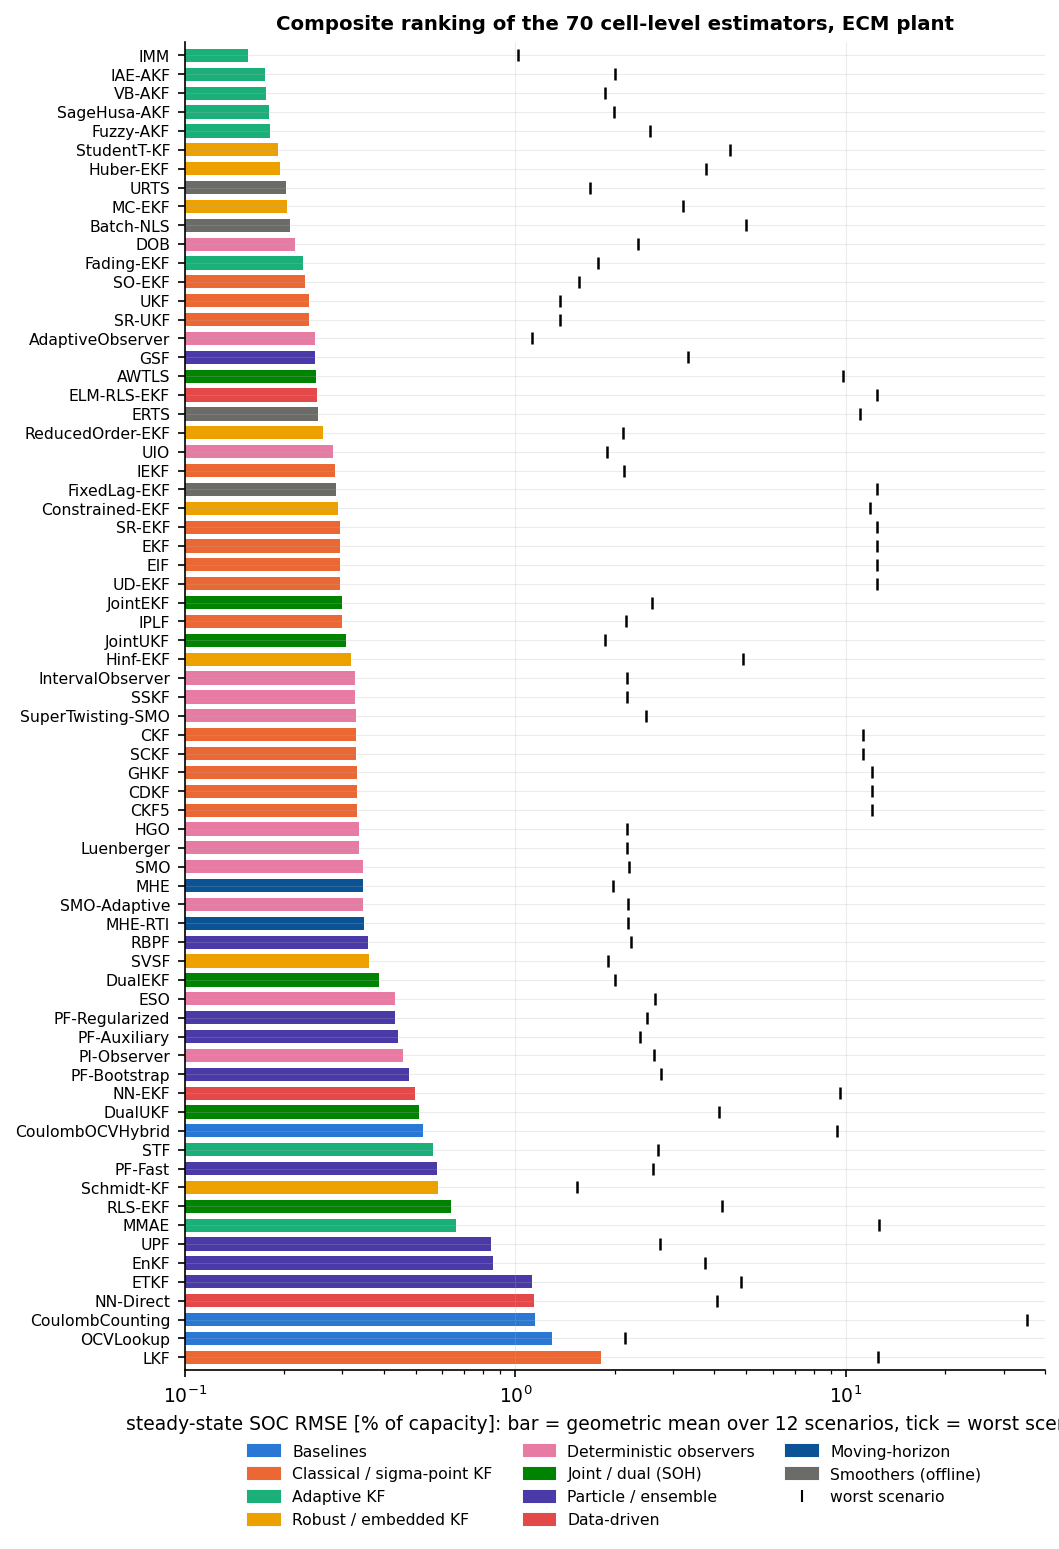
\includegraphics[width=0.95\textwidth]{figures/res_ranking_bars.png}
\caption{The composite ranking of \cref{tab:ranking} as a bar chart: geometric-mean
steady-state RMSE over the twelve scenarios (bar, log scale) with the worst-scenario RMSE (tick).
The families interleave; the adaptive and M-estimator filters lead, and the estimators with a
worst case above \SI{10}{\percent} are the tangent-linearised Kalman filters and their
equivalents, which fail \code{combined}.}
\label{fig:res-ranking}
\end{figure}

\begin{figure}[H]\centering
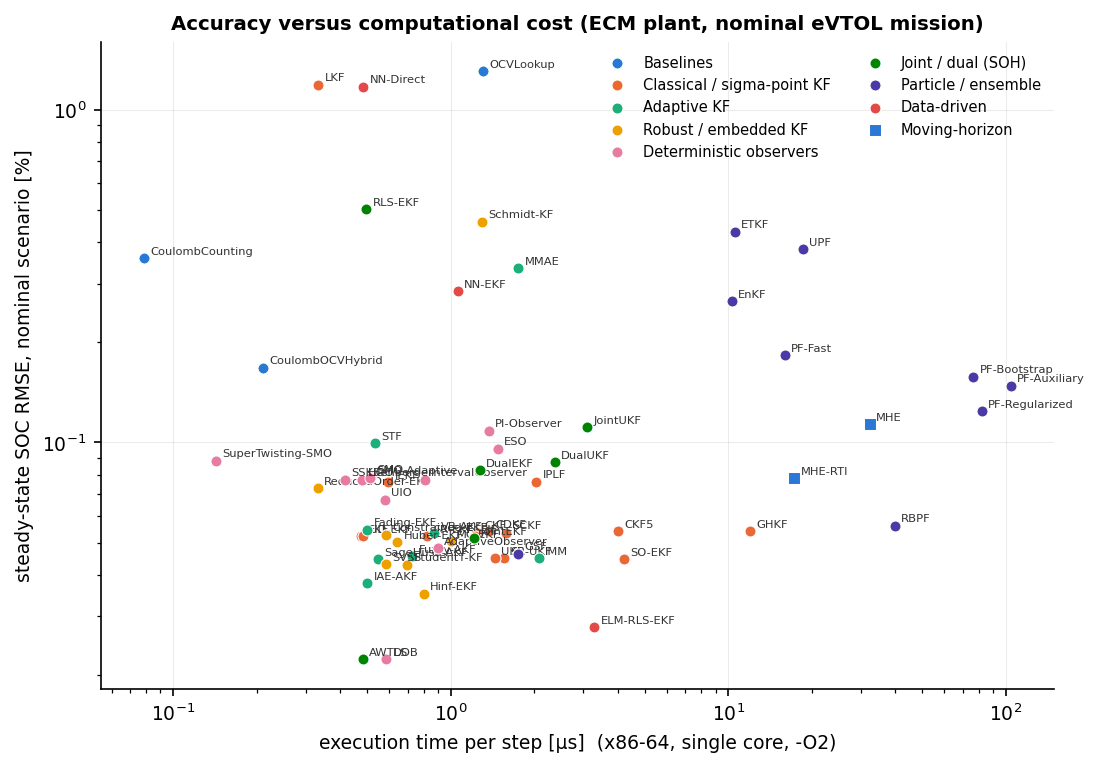
\includegraphics[width=\textwidth]{figures/overview_runtime_vs_rmse.png}
\caption{Nominal steady-state RMSE against execution time per step (x86-64, one core,
\code{-O2}, double precision). The cost axis spans three decades; the accuracy axis, for the
online estimators that are not structurally capped, spans one. The lower-left corner is
occupied by the EKF, the adaptive EKFs and the fixed-gain observers.}
\label{fig:res-runtime}
\end{figure}

\Cref{fig:res-runtime} plots nominal accuracy against cost. The Pareto front in the
(cost, geometric-mean RMSE) plane, restricted to online estimators, has six members: Coulomb
counting (\SI{79}{\nano\second}), the super-twisting sliding-mode observer
(\SI{141}{\nano\second}, \num{0.33}), the reduced-order EKF (\SI{331}{\nano\second},
\num{0.26}), AWTLS (\SI{483}{\nano\second}, \num{0.25}), the IAE-AKF (\SI{500}{\nano\second},
\num{0.18}) and the IMM (\SI{2.1}{\micro\second}, \num{0.16}). In the (cost, worst-case) plane
the front is Coulomb counting, super-twisting, reduced-order EKF, IAE-AKF, Fading-EKF
(\num{1.78} worst), the adaptive observer (\num{1.13}) and the IMM (\num{1.02}). Everything
above \SI{5}{\micro\second} per step --- the Gauss--Hermite filter, the particle filters, MHE ---
buys no accuracy on this problem that a cheaper estimator does not also deliver, with the one
exception of MHE in \code{combined} and \code{current\_bias}, where its explicit bias state is
what wins.

\section{What the equivalent-circuit results say}

Read together, the twelve columns support five statements that the rest of this Part builds
on.

The nominal problem is solved. Any correctly tuned closed-loop estimator, from a Luenberger
observer to a Gauss--Hermite filter, reaches the sensor-noise floor on a cell whose model it
knows, and the choice among them cannot be made on nominal accuracy.

Sensor faults are handled by covariance adaptation, and cheaply. The innovation-based and
Sage--Husa adaptive filters cost the same as an EKF and are the best of the field on
\code{noise\_step}, \code{outliers} and \code{sensor\_dropout}; the M-estimator filters reach
the same result with a bounded influence function and no adaptation state.

Model errors are handled by not trusting the model. On \code{aged\_cell},
\code{param\_mismatch} and \code{combined} the estimators that keep a wide covariance, carry
consider parameters, estimate the offending quantity, or have no covariance at all,
outperform the exact Bayesian filters for the wrong model. The plain EKF fails
\code{combined} not because it is a poor filter but because it is a very good one for a model
that is wrong.

Capacity requires a capacity state, and a capacity state requires excitation. Only the joint
and dual filters remove the \code{aged\_cell} error, and they are the worst of the field on the
ground-charge profile.

Cost is not a discriminator below \SI{2}{\micro\second} per step. The best twelve estimators
of the ranking all run within five times the cost of the EKF, and on a \SI{10}{\hertz} BMS
schedule even the most expensive of them uses a fraction of a percent of a
microcontroller core (\cref{ch:res-numerics}).
